\documentclass{article}
\usepackage{oconnor}
\usepackage{ wasysym }

%% UPDATE these variables:
\renewcommand{\hwnum}{2}
\title{CSCI 446, Project Design 02}
\author{Group 20: Jack Tetrault, John Hultman, Patrick O'Connor}
%%\date{due: 15 January 2021}

\begin{document}

\maketitle

CSCI 446 Artificial Intelligence

Project 02: Wumpus World

Elements of Design Document
\begin{enumerate}
    \item UML Class Diagram
    \item Textual Explanation of Major Classes in UML Diagram
    \item Major Design Decisions
    \item Experimental Design for Testing Results
\end{enumerate}
% ============================================
% ============================================
\nextprob{UML Class Diagram}

% ============================================

%\paragraph{Not needed for this project}


\begin{figure}
    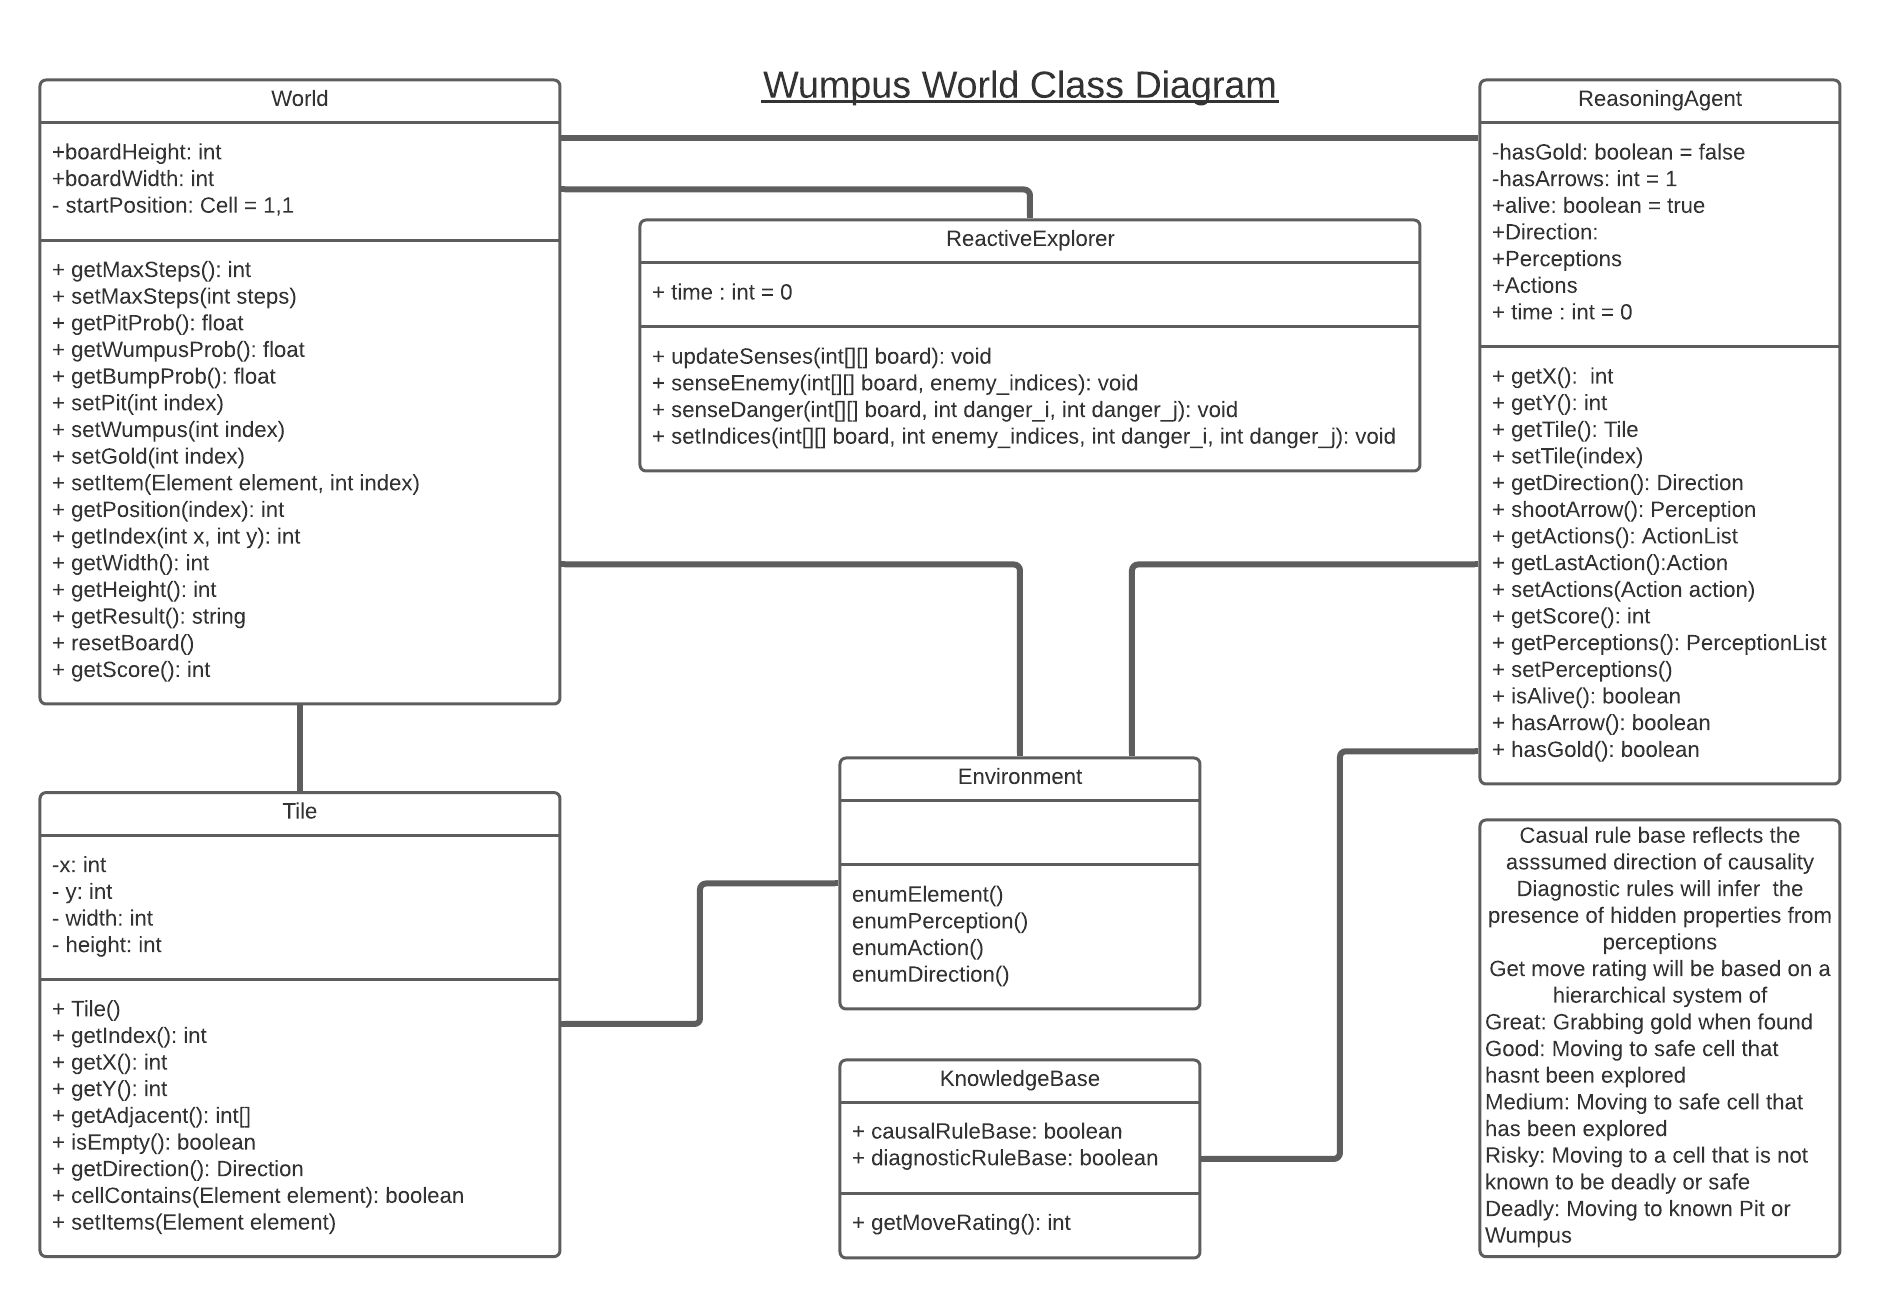
\includegraphics[width=\textwidth]{WumpusUMLDiagram.png}
    \caption{UML Drawn using Lucid App}
    \label{fig:num01}
\end{figure}
See figure \ref{fig:num01} for UML Class Diagram

% ============================================
% ============================================
\nextprob{Textual Explanation of Major Classes in UML Diagram}
% ============================================

%Paste paragraphs below here
\begin{enumerate}
    \item World: Represents the entire playable board. Provides ability to create, update, and reset game boards.
    \item Environment: Class for enumerating all of the possibilities for Elements, Perceptions, Actions, and Directions
    \item Tile: Represents the spaces in the current world. Provides the location of players, gold, pits, etc. 
    \item ReasoningAgent: Represents our player. Provides information about players location and status. This agent is capable of backtracking and utilizing data from the previous moves committed.
    \item ReactiveExplorer: Provides the player the ability to check surrounding cells and update the board with new danger information. This exploring agent is not capable of knowingly backtrack or utilizing information from previous moves besides knowing where it exists on the board.
    \item KnowledgeBase: Class for interpreting, implementing and returning the best action plan. This class will hold both the causal and diagnostic rules. Lastly for the reasoning agent each of the moves will have a ranking of either Great, Good, Medium, Risky, Deadly. Great will be grabbing the gold. Good will be moving to a safe cell that has not been explored yet. Medium will be moving to a safe cell that has already been explored. Risky will be moving to a cell that is not known to be deadly or safe. Lastly, Deadly will be moving to a known Pit, or Wumpus. For the reactive explorer, the same rating will be applied but with a reduced set that merges good and medium as it is not possible for this agent to see backwards in “time”.
\end{enumerate}



% ============================================
% ============================================
\nextprob{Major Design Decisions}
% ============================================

%Paste paragraphs below here
One major design decision we made was the implementation of the KnowledgeBase class. This class simulates the 
rationale for our player. A hierarchical system of ranking danger levels of cells is part of its functionality. 
The parameters of this class include causalRuleBase and a diagnosticRuleBase, both boolean values. Causal rule 
base reflects the assumed direction of causality. Diagnostic rules will infer the presence of hidden properties 
from perceptions. getMoveRating() returns a “move” rating based on the hierarchical system. Along with this, for 
creating the wumpus world we have decided to create a tile class instead of using a list to store the index, 
coordinates(x,y), and elements. This will allow us more flexibility and functionality that is directly related 
to the wumpus world. With regard to the rules we have established the following as of now although all of them have not 
been converted to clause form yet: 

Causal rules reflect the assumed direction of causality in the world:
\begin{itemize}
    \item  $\forall l_1,l_2,s At(Wumpus,l_1,s) \wedge Adjacent(l_1,l_2)=>Smelly(l_2)$
    \item $\forall l_1,l_2,s At(Pit,l_1,s) \wedge Adjacent(l_1,l_2)=>Breezy(l_2)$
\end{itemize}

Diagnostic rules infer the presence of hidden properties directly from the percept-derived information
\begin{itemize}
    \item  $\forall l,s At(Agent,l,s) \wedge Breeze(s) => Breezy(l)$
    \item $\forall l,s At(Agent,l,s) \wedge Stench(s) => Smelly(l)$
\end{itemize}

For Preference among the action taken by the agent
\begin{itemize}
    \item $\forall a,s Great(a,s) => Action(a,s)$
    \item $\forall a,s Good(a,s) \wedge (\lnot \exists b Great(b,s)) => Action(a,s)$
    \item $\forall a,s Medium(a,s) \wedge (\lnot \exists b Great(b,s) \lor Good(b,s)) => Action(a,s)$
    \item This cycle continues until you have to take the Deadly step.
    \item Along with this once gold is found we override the previous hierarchy and go back to start as soon as possible
    \item $\forall s Holding(Gold, s) => GoalLocation([1,1], s)$
\end{itemize}



% ============================================
% ============================================
\nextprob{Experimental Design for Testing Results}
% ============================================

%Paste paragraphs below here
Our experimental design for testing our results is to implement a reactive explorer as well as the first order 
logic explorer. Then record the number of times each explorer finds the gold, kills a wumpus, falls in a pit, 
is killed by a wumpus, and the number of cells explored. We will then compare the two and see which performs 
better on each statistic. With the more times an explorer kills a wumpus and finds gold being better. Then the 
fewer times it falls in a pit, is killed by a wumpus, and the fewer number of cells visited the better. We will 
also keep track of the total number of decisions made by both explorers and compare those with the one with less 
total decisions being better. We will run these metrics on several different cave sizes multiple different times 
to produce an average that we will then compare to make our conclusions on.



\end{document}

